% The document class supplies options to control rendering of some standard
% features in the result.  The goal is for uniform style, so some attention 
% to detail is *vital* with all fields.  Each field (i.e., text inside the
% curly braces below, so the MEng text inside {MEng} for instance) should 
% take into account the following:
%
% - author name       should be formatted as "FirstName LastName"
%   (not "Initial LastName" for example),
% - supervisor name   should be formatted as "Title FirstName LastName"
%   (where Title is "Dr." or "Prof." for example),
% - degree programme  should be "BSc", "MEng", "MSci", "MSc" or "PhD",
% - dissertation title should be correctly capitalised (plus you can have
%   an optional sub-title if appropriate, or leave this field blank),
% - dissertation type should be formatted as one of the following:
%   * for the MEng degree programme either "enterprise" or "research" to
%     reflect the stream,
%   * for the MSc  degree programme "$X/Y/Z$" for a project deemed to be
%     X%, Y% and Z% of type I, II and III.
% - year              should be formatted as a 4-digit year of submission
%   (so 2014 rather than the academic year, say 2013/14 say).

\documentclass[ % the name of the author
                    author={James Stephenson},
                % the name of the supervisor
                supervisor={Dr. Edwin Simpson},
                % the degree programme
                    degree={MSc},
                % the dissertation    title (which cannot be blank)
                     title={Project Plan: Bayesian Deep Learning For Extractive Test Summarisation},
                % the dissertation subtitle (which can    be blank)
                  subtitle={},
                % the dissertation     type
                      type={},
                % the year of submission
                      year={2022}]{../additions/dissertation}

\begin{document}

	% =============================================================================
	
	
	% =============================================================================
	
	% This macro creates the standard UoB title page by using information drawn
	% from the document class (meaning it is vital you select the correct degree 
	% title and so on).
	
	
	\maketitle
	
	% After the title page (which is a special case in that it is not numbered)
	% comes the front matter or preliminaries; this macro signals the start of
	% such content, meaning the pages are numbered with Roman numerals.
	
	\frontmatter
	
	% LaTeX automatically generates a table of contents, plus associated lists 
	% of figures, tables and algorithms.  The former is a compulsory part of the
	% dissertation, but if you do not require the latter they can be suppressed
	% by simply commenting out the associated macro.
	
	\tableofcontents
	
	% The following sections are part of the front matter, but are not generated
	% automatically by LaTeX; the use of \chapter* means they are not numbered.
	
	% -----------------------------------------------------------------------------
	
	\chapter*{Abstract}		

		Text summarisation is a valuable technique that allows for computational processing of documents, saving readers hours in manual processing. Users have different summary requirements; however, current extractive summarisation systems construct generic summaries that are not tailored to the user's needs. Asking users for feedback for summary improvement is one solution to combat this problem, yet this introduces an additional step of manual processing. Thus we look to minimise the amount of required user feedback.
		
		This project will investigate the feasibility of applying newly-developed techniques from Bayesian deep learning \cite{Wilson20} to get significant estimates of the model's confidence, so we are able to ask the user for more explanatory feedback. Legacy approaches use Bayesian optimisation \cite{Simpson19} strategies the achieve minimal user feedback. However, this strategy is blocked since modern summarisation techniques involve deep neural networks. These models cannot effectively express uncertainty and are typically overconfident when encountered by new topics \cite{Xu19}. 
		
		We will use existing exploratory frameworks \cite{Simpson19} for evaluation. 
	
	\mainmatter
	
	% -----------------------------------------------------------------------------
	 
	\chapter{Two Pages of Coherent Text: An Introduction}
	\label{chap:introduction}
		
		It should include at least two pages of coherent text (i.e., of the form you intend to write for your thesis, not rough-notes) that could be used as the opening pages of your Introduction/Overview chapter (Chapter 1 of your thesis). 
		
	% -----------------------------------------------------------------------------
	
	\chapter{Subject Background}
	\label{chap:literaturereview}
		
	Since the crux of this project is to assess the suitability of applying Bayesian deep learning (BDL) techniques to passage ranking (PR) problems, this chapter explores the relevant literature that discusses previous approaches to passage ranking solutions. Once this assessment has been done, we will then also examine literature that assesses BDL as opposed to classical deep learning techniques.
		
		\section{Interactive Learning}
		\label{chap:literaturereview:interactive}
		
		Interactive learning is a machine learning workflow involving directed experimentation with inputs and output \cite{Amershi14}. Rapid change in response to user input facilitates interactive inspection on impact of user input.  This workflow format is commonly used to solve NLP problems; related works include literature in passage ranking (PR) of generated text in the context of translations, question answering and text summarisation \cite{Peris18, Lin17, PVS17}. These works had a focus on interactionally-expensive uncertainty sampling to learn the rankings of \emph{all} candidate passages \cite{Simpson19}. Gao et al. \cite{Gao18} researched how to reduce the number of user interactions for uncertainty sampling techniques with some success using an active learner (AL). A positive step towards reasonable interactive learning.

	\medbreak
	Simpson et al \cite{Simpson19} take an alternative approach to uncertainty sampling by proposing a Bayesian optimisation (BO) strategy instead \cite{Simpson19}. With Gaussian process (GPs) displaying some success in error reduction for NLP tasks with noisy labels \cite{Cohn13, Beck14}, Simpson and Gurevych \cite{Simpson18} proposed using Gaussian process preference learning (GPPL) with uncertainty sampling. This approach has been further built upon by Simpson et al. \cite{Simpson19} to a BO framework. This approach showed a markable improvement in the accuracy of chosen answers in a community question answering (cQA) task with a small number of interactions required \cite{Simpson19}. The methodology used Expected Improvement (IMP) as the acquisition function for AL which twisted the focus of optimisation to find the best candidate, as opposed to the ranks of all candidates \cite{Simpson19}. The switch to exploitation of promising candidates showed to be massively influential on performance \cite{Simpson19}. Simpson et al. \cite{Simpson19} furthered the performance enhancement gained from using the BO framework by using prior predictions from a deep learner as an informative prior for GPPL \cite{Simpson19} to address the cold-start problem for recommender systems \cite{Bobadilla12}.

		
		\section{Active Learning}
		\label{chap:literaturereview:active}
		
		Active
		
			\subsection{Active Learning Strategies}
			\label{chap:literaturereview:active:strategies}
			
			Active Strategies
		
		\section{Deep Learning}
		\label{chap:literaturereview:deep}
		
		Deep learning methods form a subset of machine learning, based on neural networks with at least three hidden layers. These techniques have dramatically increased capabilities of model recognition in many domains including visual object recognition, question answering and text summarisation \cite{Lecun15, Sharma18, Azar17}. 
		
	%% [NN Deep Learning Image]

In classical training, one typically uses maximum a-posteriori (MAP) optimisation to choose the set of parameters, $\hat{w}$, for our model that maximises the posterior probability from our parameter distribution \cite{Wilson20}. MAP does not require the computationally-costly calculations of the marginal distribution; however, since MAP is a point estimate, it cannot be fully considered a Bayesian approach \cite{Hero15}.
	
	%% [Hero15 plot]

		
			\subsection{Pre-trained Models}
			\label{chap:literaturereview:deep:pretrained}
			
			Pre-trained, deep learning, language models are useful in unsupervised learning problems due to the lack of major architectural modifications required and the high performance levels that are delivered \cite{Mridha21}. One popular pre-trained language model is the Bidirectional Encoder Representations from Transformers (BERT) which takes an entire sequence of words at once to produce significantly improved results; with some minor fine-tuning, it can be applied to many NLP tasks \cite{Mridha21}.

Recent publications have found BERT-based models \cite{Devlin18} to be extremely effective when tasked with passage ranking situations across the question answering and text summarisation disciplines \cite{Xu19, Qiao19}. Xu et al. \cite{Xu19} explored a query-passage set up when applying BERT to cQA such that the BERT final hidden state fed into an MLP module to produce relevance scores in a supervised way. Since this technique outperformed the baseline, it may be a useful structure to consider adapting to the text summarisation domain.

The limitation of utilising an interactive learning framework such as one outlined by Simpson et al. \cite{Simpson19} as that it does not utilise the vast performance capabilities of newer, pre-trained techniques such as BERT. Although the framework presented does limit the number of interactions required from a user – allowing the user to tailor the summary – Ein-Dor et al. \cite{EinDor20} look to take this idea further with the incorporation of a BERT component in an AL framework. 

		\section{Bayesian Optimisation}
		\label{chap:literaturereview:bo}
		
		Bayesian Optimisation

		
		\section{Deep Active Learning}
		\label{chap:literaturereview:deepactive}
		
		Ein-Dor et al. \cite{EinDor20} developed a framework that used an AL approach with BERT-based classification. Zhang and Zhang also explored an alike ensemble of AL strategies \cite{Zhang19}; however, the task is less relatable to PR since framework proposed by Ein-Dor et al. had experimentation on data with high class imbalance, scarce labelling and a small annotation budget \cite{EinDor20}, attributes of an interactive PR context.  This structure consisted of pool-based AL \cite{Settles09} in batch mode in conjunction with BERT as the classification scheme. Different AL strategies were examined – Monte-Carlo Dropout (MCD) \cite{Gal15}, a Bayesian approach, and Discriminative Active Learning (DAL) \cite{Gissin19} – with Al proving an excellent boost to helping BERT emerge from its poor initial model \cite{EinDor20}. Although DAL would not be appropriate for the PR context due to its focus on querying batches, using MCD as a strategy is a technique we could consider.
		
		\section{Bayesian Deep Learning}
		\label{chap:literaturereview:deepbayes}
		
		Deep bayes
		
			\subsection{Bayesian Deep Learning Strategies}
			\label{chap:literaturereview:deepbayes:strategies}
			
			Deep Bayes Strategies

		
		% ----------------------------------------------------------------------------	
	
	% =============================================================================
	
	% Finally, after the main matter, the back matter is specified.  This is
	% typically populated with just the bibliography.  LaTeX deals with these
	% in one of two ways, namely
	%
	% - inline, which roughly means the author specifies entries using the 
	%   \bibitem macro and typesets them manually, or
	% - using BiBTeX, which means entries are contained in a separate file
	%   (which is essentially a database) then imported; this is the 
	%   approach used below, with the databased being dissertation.bib.
	%
	% Either way, the each entry has a key (or identifier) which can be used
	% in the main matter to cite it, e.g., \cite{X}, \cite[Chapter 2}{Y}.
	
	\backmatter
	
	\bibliography{bibtex}
	
	% -----------------------------------------------------------------------------
	
	% The dissertation concludes with a set of (optional) appendices; these are 
	% the same as chapters in a sense, but once signalled as being appendices via
	% the associated macro, LaTeX manages them appropriately.
	
	\appendix
	
	\chapter{Time-plan}
		\label{appx:timeplan}
		
		\begin{center}
			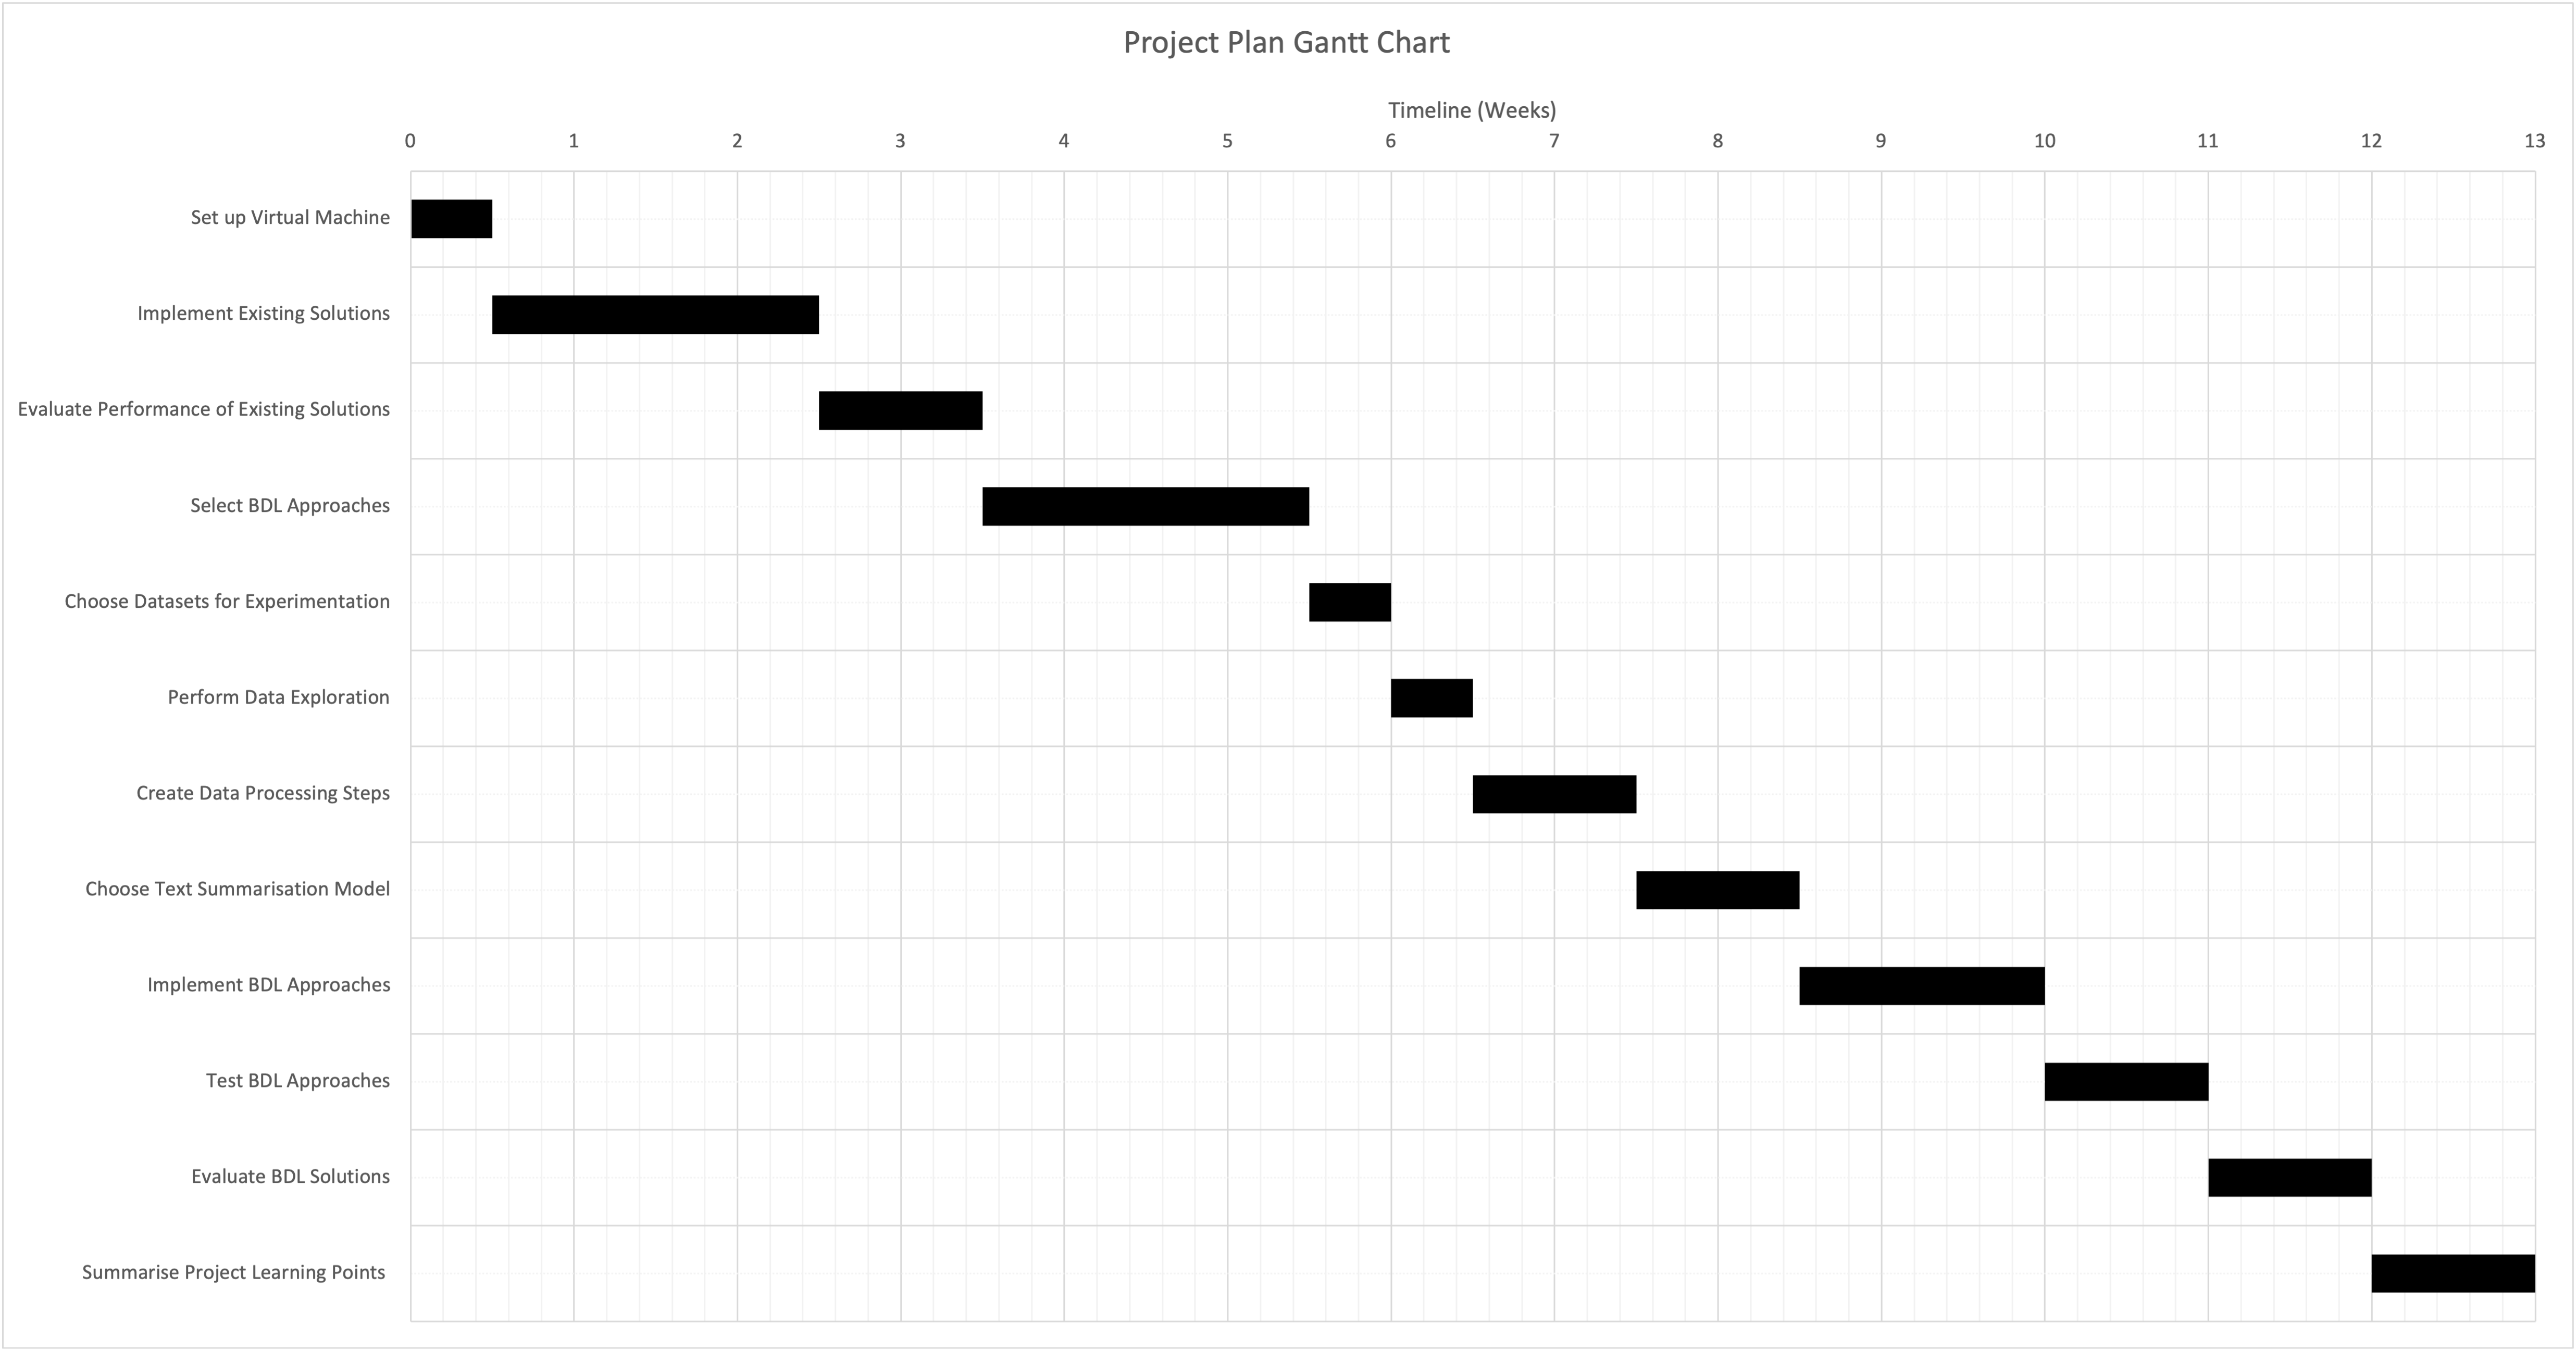
\includegraphics[width=\textwidth,height=\textheight,keepaspectratio]{Gantt.png}
		\end{center}
		
	\chapter{One-Page Risk Assessment}
		\label{appx:riskassessment}
		
		It should include as an Appendix a one-page risk assessment for your project, talking about the major risks you can foresee that might plausibly occur and interfere with your plans. For each risk, state clearly what it is, what its likelihood is, what its effects/impact would be on the project, and what your intended mitigation or risk-reduction involves.
		
		% =============================================================================

\end{document}
